\chapter{The Three-Terminal Black Box}

\section*{Objectives}

\begin{enumerate}
\item To study a three-terminal black box and identify the circuit within it along with the values of the electronic components.

\item To understand the responses of different active and passive circuit elements and their combinations, and to learn to recognise them.

\item To exercise your deductive and inductive powers, much as real physicists must do with real experiments.
\end{enumerate}


\section*{Introduction}

You are given a sealed box with three terminals marked $A$, $B$, and $C$ which connect to a circuit inside. This circuit consists of \textbf{three} electronic components of different kinds, arranged between the three terminals in either a ``star'' or ``delta'' connection, as shown in Figure (\ref{fig:bb}). You are expected to identify each component's type, value, and orientation with respect to the terminals. 

\begin{figure}[!htb]
    \centering
    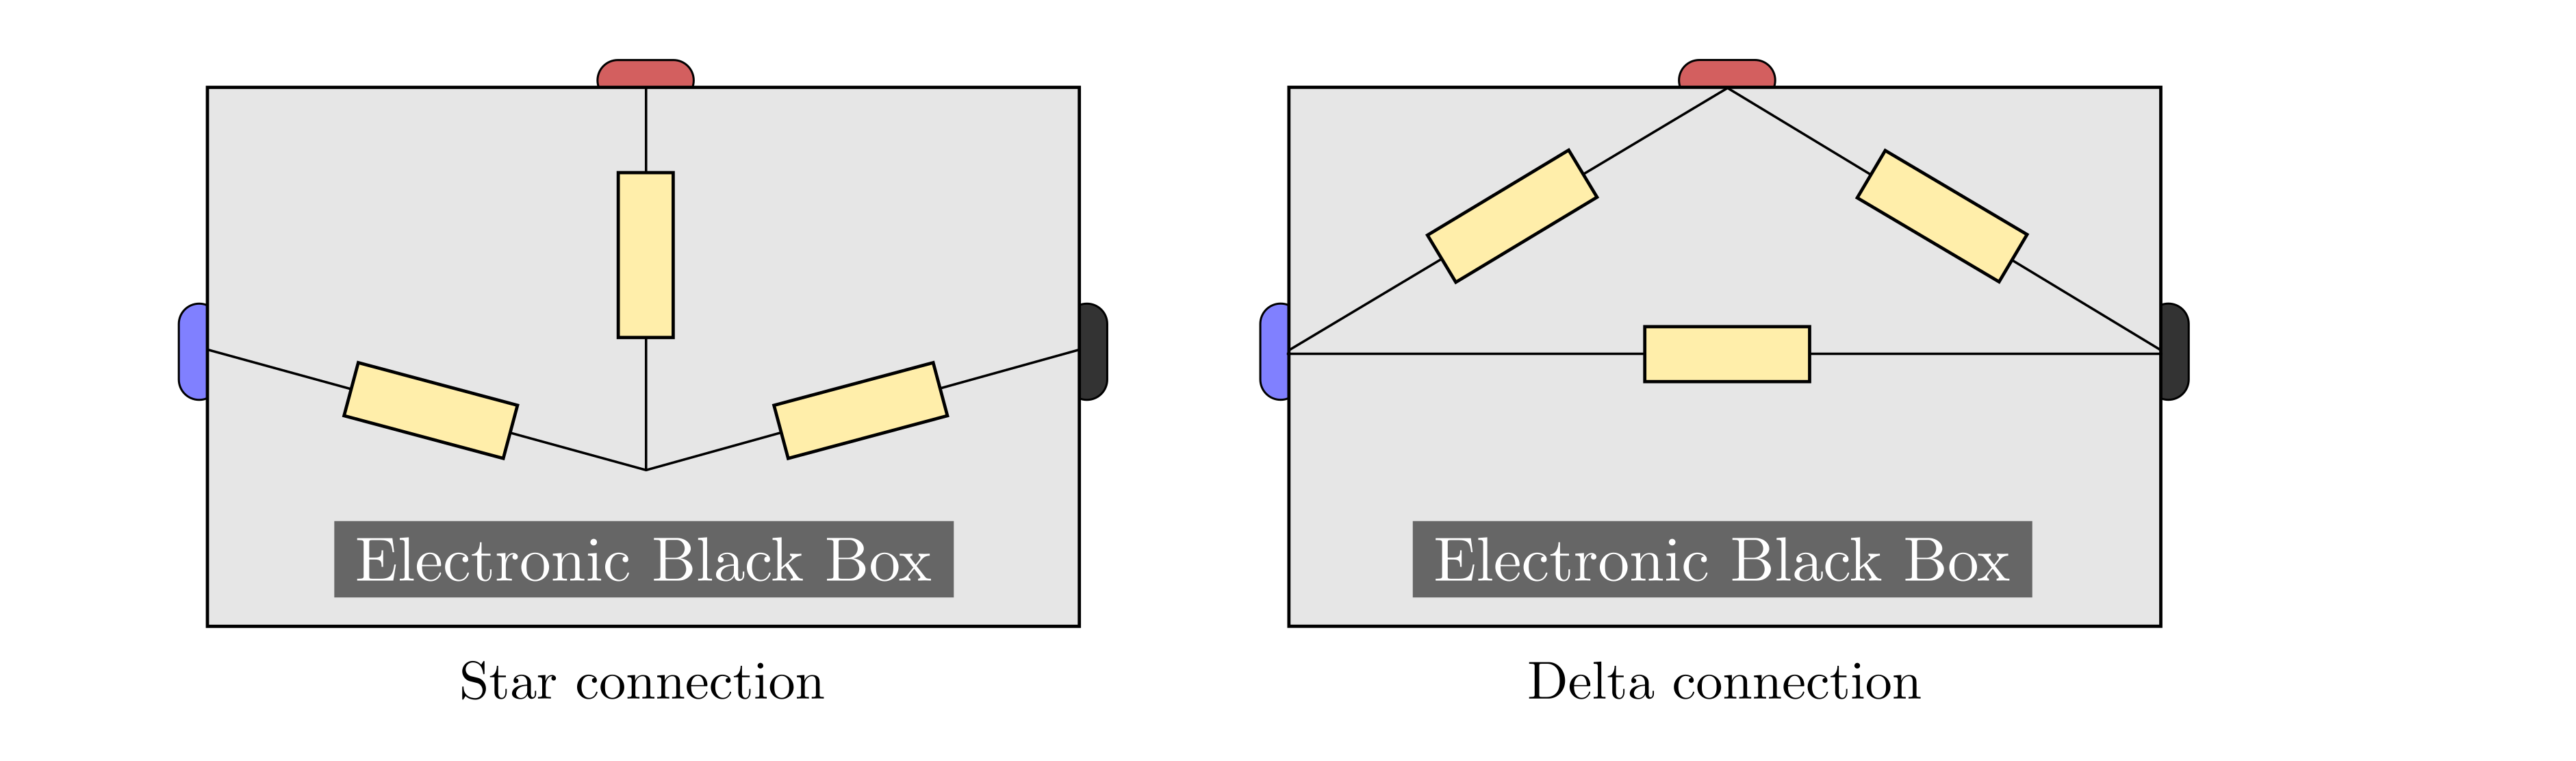
\includegraphics[scale=0.3]{figs/bb.png}
    \caption{Different configurations possible within a blackbox: it will be specified if the box contains a star (\textit{left}) or delta (\textit{right}) connection. Do not attempt to open the box! }
    \label{fig:bb}
\end{figure}

\begin{imp}
You will be told beforehand if the connection is ``star'' or ``delta'' as you cannot distinguish them otherwise. This is because, if the circuit contains only resistors, every star connection has an equivalent delta connection and vice versa.

The black box will always contain \textbf{three} electronic components, but they need not all be distinct. Some components may be repeated; a black box may be composed of (i) three resistors, (ii) two resistors and a diode, (iii) a battery and two diodes, and so on. Each arm (see Figure (\ref{fig:bb})) may contain anything from all to none of the components.
\end{imp}


\subsection*{Star and Delta Connections}

Standard 3-component circuits take on two major forms with names that represent the way in which the components are connected: a \textbf{Star} sometimes represented by Y, and a Delta connected network sometimes represented by a triangle or $\Delta$.

\begin{figure}[!htb]
       \begin{subfigure}[t]{0.3\textwidth}
				\centering
                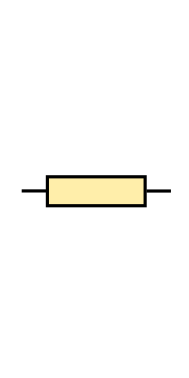
\includegraphics[scale=0.4]{bb-comp.png}
                \captionsetup{justification=centering}
                \caption{Component or combination \\of components}
       \end{subfigure}%
       \begin{subfigure}[t]{0.3\textwidth}
				\centering
                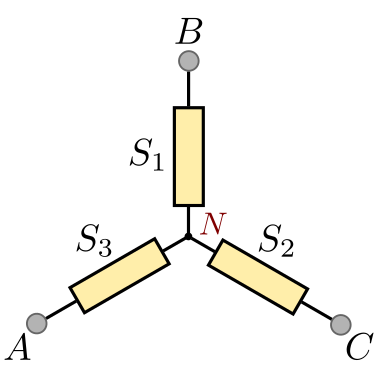
\includegraphics[scale=0.4]{bb-star.png}
                \caption{Star connection}
        \end{subfigure}%
        \begin{subfigure}[t]{0.3\textwidth}
        		\centering
                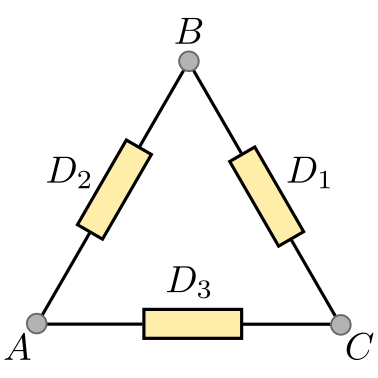
\includegraphics[scale=0.4]{bb-delta.png}
                \caption{Delta connection}
        \end{subfigure}%
        \caption{In a star connection, one node is inaccessible and so only two components are connected at any time. In a delta connection, all the components are connected.}
        \label{fig:starAndDelta}
\end{figure}

\begin{figure}[!htb]
\centering
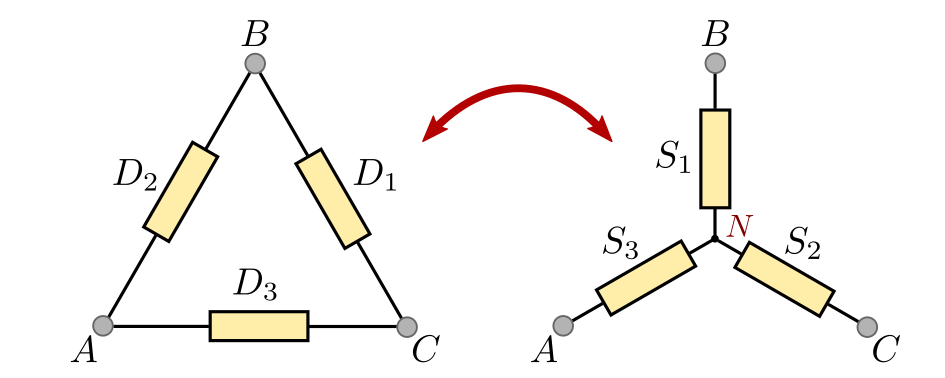
\includegraphics[scale=0.4]{figs/bb-starToDelta.png}
\caption{Every star connection has an \textit{equivalent} delta connection. If the components happen to be resistors, explicit formulae may be derived for each arm.}
\label{fig:starToDelta}
\end{figure}

 Both these forms, represented in Figure (\ref{fig:starAndDelta}), are indistinguishable from each other, in that for every star connection there is an equivalent delta connection (with different values for the individual components) and vice versa. It is for this reason that you must keep in mind what form circuit in the black box has before drawing any conclusions.

\begin{imp}
If all the components are resistances, the following formulae will allow you to move between a star connection and its associated delta connection and vice versa:

\begin{minipage}{0.5\textwidth}
\centering
\paragraph*{Delta to Star Network:}
\begin{equation*}
\begin{aligned}
P &= \frac{A B}{A + B + C}\\
Q &= \frac{A C}{A + B + C}\\
P &= \frac{B C}{A + B + C}\\
\end{aligned}
\end{equation*}
\end{minipage}
\begin{minipage}{0.5\textwidth}
\centering
\paragraph*{Star to Delta Network:}
\begin{equation*}
\begin{aligned}
A &= \frac{P Q + Q R + R P}{R}\\
B &= \frac{P Q + Q R + R P}{Q}\\
C &= \frac{P Q + Q R + R P}{P}\\
\end{aligned}
\end{equation*}

\end{minipage}

\end{imp}

\subsection*{Passive circuit components}

Passive circuit components are electrical components that cannot control the current in a circuit. They do not generate energy, but instead dissipate or store it.

\begin{description}
\item[Resistors] A resistor is an electronic component used to oppose or limit the current in a circuit. It's behaviour is dictated by Ohm’s law, which states that the voltage applied across the terminals of a resistor is directly proportional to the current flowing through it, with the constant of proportionality called the \textit{resistance}, $V=IR$.

% \begin{equation*}
% V = I R
% \end{equation*}

\item[Capacitors]

A capacitor, made from two conductive plates with an insulator between them, stores electrical energy in the form of an electric field. It blocks DC signals (when fully charged) and allows the AC signals to pass through it. The charge stored in a capacitor is given by $Q=CV$.

% \begin{equation*}
% Q = CV
% \end{equation*}

When used with a resistor, the time a capacitor takes to charge or discharge is measured in units of an intrinsic time scale, known as the time constant $\tau = RC$ of the circuit.

\end{description}



\subsection*{Active circuit components}
An active device is any type of circuit component with the ability to electrically control electron flow in the circuit.

\begin{description}
\item[Batteries]

Charges can be separated to produce a voltage. A battery uses a chemical reaction to produce energy and separate opposite sign charges onto its two terminals. As the charge is drawn off by an external circuit, doing work and finally returning to the opposite terminal, more chemicals in the battery react to restore the charge difference and the voltage.


\item[p-n junction Diodes]

These are two-terminal semiconductor devices, which allow the electric current in only one direction while blocking it in the reverse direction. A diode has an anode (or positive end) containing positive charge carriers called ``holes'', and a cathode (or negative end) containing negative charge carriers (electrons). The interface between these ends forms a region without any charge carriers called the \textbf{depletion layer}. 

The process of applying the external voltage to a p-n junction semiconductor diode is called biasing. If the diode is \textbf{forward biased} -- that is, when a positive voltage is applied to the anode and a negative voltage to the cathode -- it allows the charge carriers, and hence current, to flow. On the other hand, if the diode is \textbf{reverse biased} -- negative to the anode and positive to the cathode -- it blocks the current flow. In the conventional symbol for a diode, the arrowhead indicates the conventional direction of electric current when the diode is forward biased.

\begin{figure}[!htb]
\centering
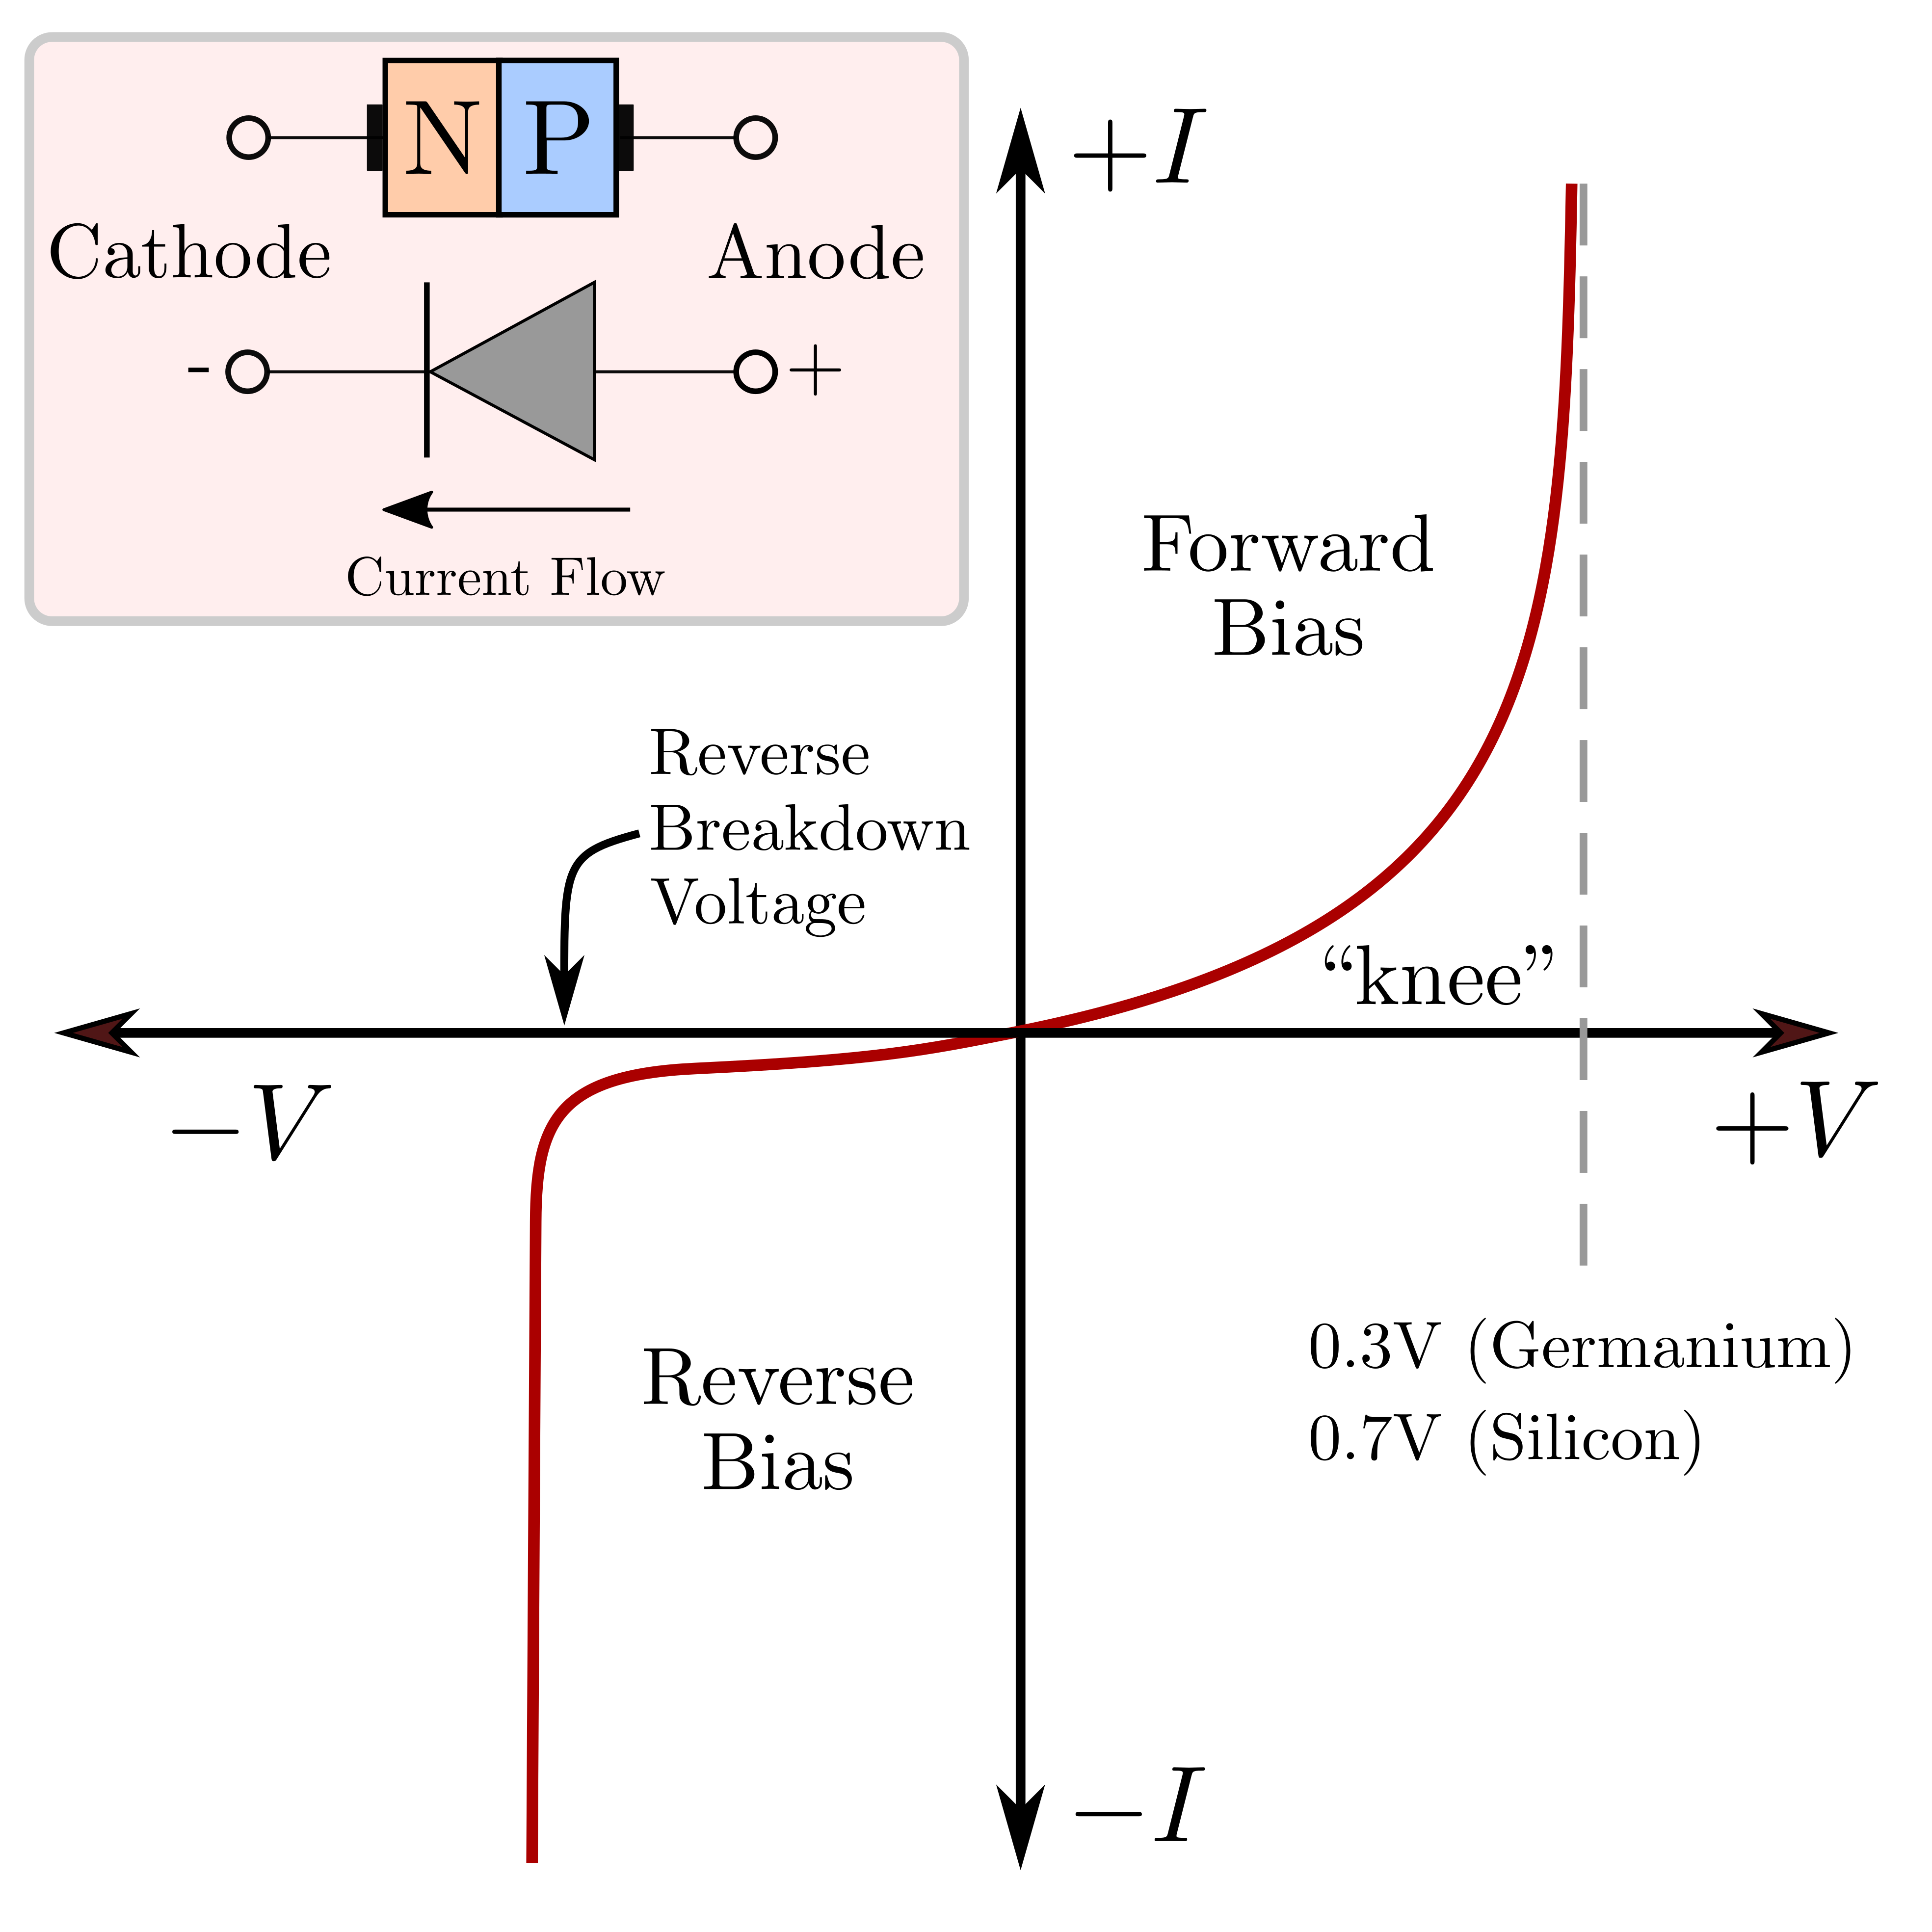
\includegraphics[scale=0.4]{figs/diode_characteristics.png}
\caption{A diode and its current-voltage characteristics: for small (positive) values of input voltage, the output current varies exponentially.}
\label{fig:diodeChar}
\end{figure}

Unlike a resistor, a diode does not behave linearly with respect to the applied voltage as the diode has an exponential current-voltage (I-V) relationship and therefore cannot be described by simply using an equation such as Ohm’s law. The reason for this is that the width of the depletion layer decreases with increase in positive voltage. After a certain ``knee'' voltage (0.3 V for Germanium semiconductors and 0.7 V for Silicon semiconductors) the width of the barrier effectively goes to zero, and the diode acts like a short circuit with zero resistance. When a junction diode is reverse biased the thickness of the depletion region increases and the diode acts like an open circuit blocking any current flow (except for a very small leakage current), until an ``avalanche'' voltage when the device undergoes a breakdown and gets shorted, leading to maximum current flow in the \textit{opposite} direction.


\end{description}




\section*{Experimental Setup}

\subsection*{Apparatus}

\begin{enumerate}
\item A black box with three connecting terminals marked $A$, $B$, and $C$
\item A variable DC power supply (\textit{Keltronix})
\item Two digital multimeters (\textit{MECO 603})
\item A signal generator (\textit{Testronix 72})
\item A Digital Storage Oscilloscope (\textit{GW INSTEK–GDS-1102U})
\item A digital stopwatch (\textit{Racer})
\item A resistor ladder
\item Connecting wires

\end{enumerate}

\subsection*{Description}

\begin{description}
\item[Digital Multimeter (\textit{MECO 603})]

A multimeter is an instrument used to measure multiple parameters like voltage, current, and resistance. In this experiment you will use the given digital multimeters (Model \textit{MECO - 603}) \textbf{\textit{only}} for the measurement of DC and AC voltage and current. You will have to use input sockets marked COM, V/$\Omega$ and mA (or 20A) for the required measurements. Note that there are two input sockets marked mA and 20A for the current measurement. The socket marked mA may be used for measuring current below 250 mA and socket marked 20A may be used for measuring current up to 20 A. You will have to select the appropriate function and the range using the rotary switch provided on the multimeter. The value of voltage or current is displayed on the LCD screen. The multimeter is turned off by turning the dial to the appropriate setting.

\item[Variable DC Power Supply (\textit{Keltronix})]

The DC Variable Power Supply can either act as a source of constant voltage (CV), or constant current (CC), indicated by the two LEDs present on it. We will be using it as a constant voltage source, so make sure the CV LED is lit. An ideal voltage source is one that produces a fixed voltage irrespective of the current the load (your circuit) demands of it. Of course, this is not realistic; the supply given to you can supply a maximum potential difference of 15V, and a maximum current of 1A.

The voltage and the current in the circuit can be changed using the three knobs: voltage coarse, voltage fine, and current. The given power supply also displays the values of the output voltage and current. Do not use these values since the multimeter will be more reliable. 

If the current knob is set to maximum, the supply acts as a constant voltage source. The constant voltage it supplies can be varied using the voltage knobs, and is independent of the load (your circuit) attached to it.\footnote{Similarly, if the voltage knob is set to maximum, the supply acts as a constant current source.}

\begin{imp}
If the current your circuit draws at any voltage is beyond 1A, the power supply will not be able to supply it. This could happen if you short the two terminals of the power supply (don't!) or if you are close to the knee voltage of a diode (as in this case, the circuit has effectively zero resistance). In this case, the power supply's LED will shift from CV to CC, indicating that it is providing the maximum current possible. Avoid this situation, as it could damage the power supply.
\end{imp}

\item[Signal Generator (\textit{Testronix 72})]

A signal generator is used to generate simple repetitive waveforms in the form of an alternating electrical wave. Typically, it will produce simple waveforms like sine, square, and triangular waves, and will allow you to adjust the frequency and amplitude of these signals. The instrument given to you generates sine and square waveforms. The output may be taken from the respective output sockets. The frequency can be adjusted by turning the dial and selecting the appropriate Frequency Multiplier button. For example, turning the dial to 3 and selecting the 10k button would provide an output waveform with a frequency of 30kHz. Similarly the amplitude switch, used in conjunction with the appropriate buttons, can be used to adjust the amplitude of the output waveform from 0V to 30V.

\end{description}




\subsection*{Precautions}

\begin{itemize}
\item The use of a multimeter to measure the resistance is strictly prohibited.
\item Do not try to open the black box, use only terminals $A$, $B$, and $C$ for the connections.
\item Passing more current through the multimeter's (250 mA or 20A) sockets than they can handle will cause its fuses to burn out, leading to an open circuit. Use an appropriate resistance to limit the current in the circuit. The current should not exceed 500 mA.
\item \textbf{Do not} short the outputs of the power supply, it could damage the equipment.

\item When drawing circuit diagrams use the standard symbols.
\item The digital multimeter, the DC power supply or the signal generator should be turned off if not in use.

\end{itemize}


\section*{Procedure}

\subsection*{Part A}

The black box will contain only combinations of resistors, p-n junction diodes, and batteries in a \textit{\textbf{star}} connection.

\begin{question}
    \paragraph{Question:} Since not all of the elements will necessarily be present in a box, which is the first element you will test for?
    \end{question}

\begin{enumerate}
    \item Choose the first element that you would like to detect (or eliminate), and design a method to do this.
    
    
    \item Repeat this for all the components.
    
    \begin{question}
    \paragraph{Question:} How could you tell which way a diode was oriented? 

    \paragraph{Question:} How would you differentiate between a diode and a resistor?
\end{question}
    
    \item Give your answer in the form of a circuit diagram showing the terminals $A$, $B$, and $C$ clearly. 
\end{enumerate}

\begin{tip}
You will need to give \textit{all} the information required in order to reconstruct the circuit. For example, you will need to determine the values of the resistors, the orientation of the diodes, and the voltage and orientation of the battery, if any of the above are used in the circuit.
\end{tip}

\begin{imp}
Clearly report the procedural steps you have taken with reference to (i) your complete plan of experiment, (ii) the data you will collect, (iii) how the collected data will be analysed and (iv) how your analysis will be interpreted. Your reporting should be comprehensive, and all important steps should be mentioned in your answer sheet.
\end{imp}

\subsection*{Parts B, C, \& D \textit{(optional)}}

\begin{itemize}
    \item \textbf{Part B:} The black box will contain only combinations of resistors, p-n junction diodes and capacitors in a \textit{\textbf{star}} connection. 
    
    \item \textbf{Part C:} The black box will contain only combinations of resistors, p-n junction diodes, and batteries in a \textit{\textbf{delta}} connection. 
    
    \item \textbf{Part D:} The black box will contain only combinations of  resistors, capacitors, and inductors in a \textit{\textbf{star}} connection.
\end{itemize}

% \subsection*{Part C \textit{(optional)}}
% The black box will contain only combinations of resistors, p-n junction diodes, and batteries in a \textit{delta} connection. 

% \subsection*{Part D \textit{(optional)}}
% The black box will contain only combinations of  resistors, capacitors, and inductors in a \textit{star} connection.


\section*{References}

\begin{enumerate}

\item \href{https://www.elprocus.com/major-electronic-components/}{Overview of Various Basic Electronics Components.} Retrieved June 28, 2019, from (\nolinkurl{https://www.elprocus.com/major-electronic-components/})

\item \href{https://www.electronics-tutorials.ws/dccircuits/dcp_10.html}{Star Delta Transformation.} Retrieved June 28, 2019, from \nolinkurl{https://www.electronics-tutorials.ws/dccircuits/dcp_10.html} 

\item \href{https://www.electronics-tutorials.ws/diode/diode_3.html}{Electronics Tutorials: PN Junction Diode.} Retrieved June 28, 2019, from \nolinkurl{https://www.electronics-tutorials.ws/diode/diode_3.html}

\end{enumerate}


\newpage